I decompose the TOU-tariff-causing reductions in household electricity consumption during the peak rate period into two parts to determine the share of energy savings stemming from two different sources: savings from non-temperature-control and temperature-control uses. Here, the non-temperature-control-related electricity savings mean the stable savings that occur every day regardless of each day's heating degrees. That is, the savings associated with non-temperature-control electricity use do not vary across days. On the contrary, the latter savings strictly depend on HDDs, which fluctuate daily. Therefore, the temperature-control-related electricity savings are additional savings that appear on days with positive HDDs due to reductions in electricity consumption for heating. Isolating the impact of TOU prices on household electricity demand for temperature-control use from the total reductions in electricity demand enables us to know how differently the TOU tariff structures function from day to day, whose implications will be discussed in the next section.

To break down peak-hours household responses to TOU prices, I exploit the following econometric model inspired by the DID framework:
\begin{equation}
\begin{split}
    \textit{kWh}_{ith} \ 
    & = \ \beta_{1} \textit{HDD}_{t} \ + \ \beta_{2} \textit{HDD}_{t} \cdot \mathbb{1}\left[ \text{Treatment} \right]_{i} \\ 
    & \hspace{0.7cm} + \ \beta_{3} \mathbb{1}\left[ \text{Post} \right]_{t} \ + \ \beta_{4} \textit{HDD}_{t} \cdot \mathbb{1}\left[ \text{Post} \right]_{t} \\ 
    & \hspace{0.7cm} + \ \beta_{5} \mathbb{1}\left[ \text{Treatment \& Post} \right]_{it} \ + \ \beta_{6} \textit{HDD}_{t} \cdot \mathbb{1}\left[ \text{Treatment \& Post} \right]_{it} \\ 
    & \hspace{0.7cm} + \ \alpha_{iw} \ + \ \gamma_{dw} \ + \ \delta_{m} \ + \ \epsilon_{ith}
\end{split}
\label{Eq:Model-Specification_Breakdown-of-Hourly-Average-Treatment-Effect}
\end{equation}
Like (\ref{Eq:Model-Specification_Hourly-Average-Treatment-Effects}), the dependent variable $kWh_{ith}$ is the electricity consumption by household $i$ on the day $t$ during the hour of the day $h$. There are three indicator variables in the model: the first indicator variable $\mathbb{1}[\text{Treatment}]_{i}$ has the value of 1 if household $i$ is assigned to the treatment group; the second indicator variable $\mathbb{1}[\text{Post}]_{t}$ equals 1 when the day $t$ is in the treatment period; the last indicator variable $\mathbb{1}[\text{Treatment \& Post}]_{it}$ is equal to 1 only for treatment households during the treatment period. The model also includes interaction terms between daily HDDs and those indicator variables. The terms $\alpha_{iw}$, $\gamma_{dw}$ and $\delta_{mw}$ are household-by-half-hourly-time-window, day-of-week-by-half-hourly-time-window and month-of-year-by-half-hourly-time-window fixed effects, respectively. 

The primary coefficients of interest in (\ref{Eq:Model-Specification_Breakdown-of-Hourly-Average-Treatment-Effect}) are $\beta_{5}$ and $\beta_{6}$. Both coefficients show how much electricity consumption households have reduced since the deployment of the TOU tariffs. To be specific, $\beta_{5}$ is the decrease in household electricity consumption for non-temperature-control uses, while $\beta_{6}$ is associated with the reductions in electricity consumed to satisfy household heating needs for given HDDs. 

Using the points estimates of the two coefficients of interest presented in Table \ref{Table:Breakdown-of-Average-Treatment-Effects-in-the-Peak-Rate-Period}, I show how the electricity savings caused by the TOU prices vary with daily HDDs in Figure \ref{Figure:Breakdown-of-Hourly-ATEs-in-the-Peak-Rate-Period}.\footnote{In Table \ref{Table:Breakdown-of-Average-Treatment-Effects-in-the-Peak-Rate-Period}, the second column demonstrates the estimates $\hat{\beta}_{5}$ and $\hat{\beta}_{6}$ obtained from the econometric model (\ref{Eq:Model-Specification_Breakdown-of-Hourly-Average-Treatment-Effect}). The first and the third columns are for robustness checks. As shown in the first column, adding household-level FEs instead of the indicator variable for assignment to the treatment group leads to the almost same regression result. The third column indicates that excluding covariates associated with the indicator variable for the treatment period results in very minimal changes in point estimates.} The figure clearly demonstrates that the households assigned to the treatment group significantly reduced their electricity consumption when they were subject to the TOU prices. Specifically, they reduced their consumption by about 10\% on a day with zero HDD. In addition, it is evident from the figure that the share of temperature-control-use-related demand reductions grows as household electricity needs for heating become serious. For example, the energy savings originating from electricity consumption for temperature-control use were close to half of the total TOU-pricing-inducing reductions in household electricity demand when Irish household needs for heating were at their peak (i.e., around daily HDDs of 35).  

\begin{figure}[!th]
\centering
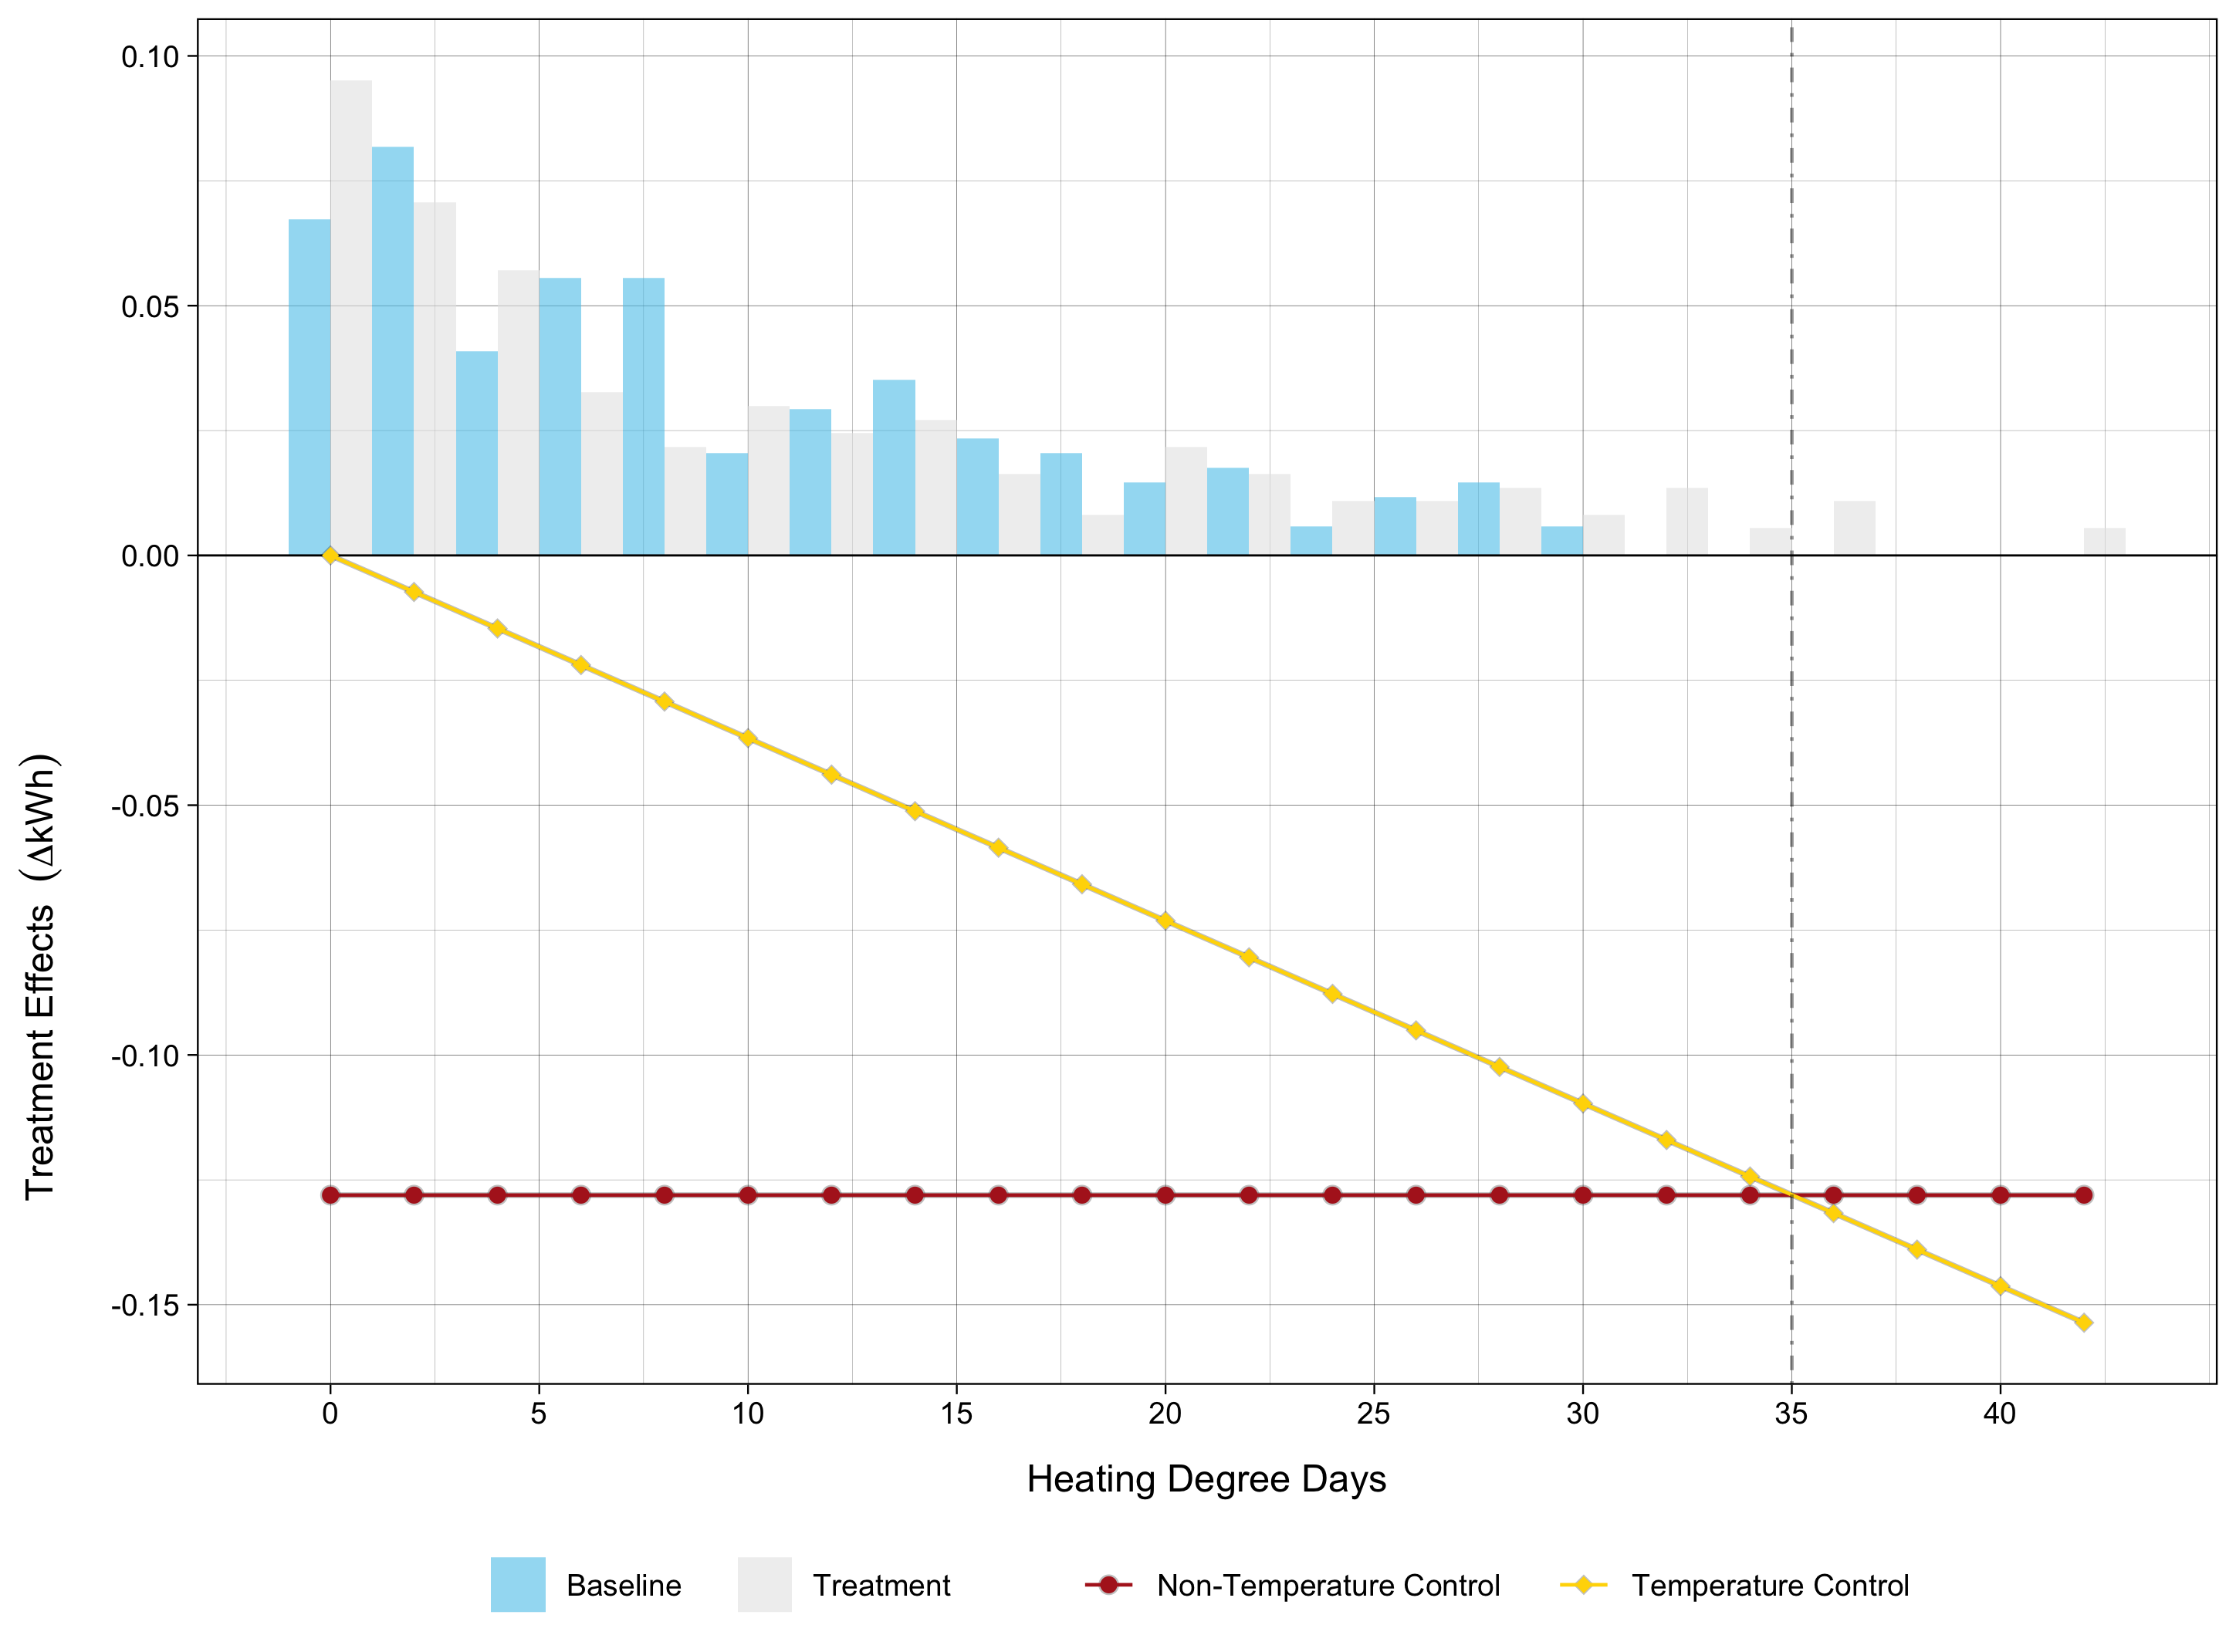
\includegraphics[scale = 0.16]{03_Chapter-2/00A_Figures/Figure_Breakdown-of-Hourly-ATEs-in-the-Peak-Rate-Period.png}
\caption{Breakdown of Hourly Average Treatment Effects}
\label{Figure:Breakdown-of-Hourly-ATEs-in-the-Peak-Rate-Period}
\end{figure}

The specification (\ref{Eq:Model-Specification_Breakdown-of-Hourly-Average-Treatment-Effect}) is also utilized to examine the relationship between the degree of price increases and the electricity savings during the peak rate period. The point estimates of coefficients of interest, demonstrated in the last four columns of Table \ref{Table:Breakdown-of-Average-Treatment-Effects-in-the-Peak-Rate-Period}, are interesting in two points. First, the reduction in non-temperature-control electricity demand caused by introducing the TOU tariffs is positively proportional to the size of the change in price during peak hours. In other words, the electricity savings occurring on any day regardless of the average daily temperatures obviously follow the law of demand. Second, the savings associated with temperature-control electricity use are insensitive to the price jumps in the peak rate period. 

\begin{table}[!th]
% Add the title
\caption{Breakdown of Average Treatment Effects in the Peak Rate Period}
\label{Table:Breakdown-of-Average-Treatment-Effects-in-the-Peak-Rate-Period}
\centering
% Determine font size
\small
% The number of "c" is equal to the number of columns. And determine the width
% of each column.
\begin{adjustbox}{scale = 0.8}
\begin{tabular}{@{\extracolsep{5pt}}lccccccc}
\\[-5.5ex]
\hline \hline
\\[-3.0ex]
% Add the label of the dependent variable. And the number must be the same with
% the number of columns.
& \multicolumn{7}{c}{Hourly Electricity Consumption  (kWh/Hour)} \\
\\[-3.0ex]
% The range must be "2-(The number of columns + 1)"
\cline{2-8}
\\[-3.0ex]
%& All & All & All & Tariff A & Tariff B & Tariff C & Tariff D \\
%\\[-4.0ex]
& (1) & (2) & (3) & (4) & (5) & (6) & (7) \\
\\[-3.0ex]
\hline
\\[-2.0ex]
HDDs & 0.005$^{**}$ & 0.005$^{**}$ & 0.004$^{**}$ & 0.004$^{*}$ & 0.006$^{***}$ & 0.006$^{**}$ & 0.007$^{***}$ \\
& (0.002) & (0.002) & (0.002)  & (0.002) & (0.002) & (0.002) & (0.002) \\
& & & & & & & \\
$\mathbb{1}$[Treatment] & 0.077$^{***}$ & & \\
& (0.030) &  & \\
& & & & & & & \\
$\mathbb{1}$[Treatment] $\times$ HDDs & 0.003$^{**}$ & 0.003$^{**}$ & 0.004$^{**}$ & 0.005$^{***}$ & 0.004 & 0.002 & 0.001 \\
& (0.001) & (0.002) & (0.002) & (0.002) & (0.003) & (0.002) & (0.002) \\
& & & & & & & \\
$\mathbb{1}$[Post] & 0.001 & 0.001 & & 0.00002 & 0.002 & 0.001 & 0.001 \\
& (0.018) & (0.019) & & (0.019) & (0.019) & (0.019) & (0.019) \\
& & & & & & & \\
$\mathbb{1}$[Post] $\times$ HDDs & $-$0.001 & $-$0.001 & & $-$0.0005 & $-$0.001 & $-$0.001 & $-$0.001 \\
& (0.002) & (0.002) & & (0.002) & (0.002) & (0.002) & (0.002) \\
& & & & & & & \\
$\mathbb{1}$[Treatment \& Post] & $-$0.128$^{***}$ & $-$0.128$^{***}$ & $-$0.127$^{***}$ & $-$0.099$^{***}$ & $-$0.122$^{***}$ & $-$0.138$^{***}$ & $-$0.182$^{***}$ \\
& (0.015) & (0.016) & (0.015) & (0.019) & (0.026) & (0.019) & (0.025) \\
& & & & & & & \\
$\mathbb{1}$[Treatment \& Post] $\times$ HDDs & $-$0.004$^{***}$ & $-$0.004$^{***}$ & $-$0.004$^{***}$ & $-$0.004$^{***}$ & $-$0.005$^{***}$ & $-$0.003$^{*}$ & $-$0.003 \\
& (0.001) & (0.001) & (0.001) & (0.001) & (0.002) & (0.001) & (0.002) \\
& & & & & & & \\
\hline
\\[-2.0ex]
Tariff Group & All & All & All & A & B & C & D \\
FEs: ID by Half-Hourly Time Window & No & Yes & Yes & Yes & Yes & Yes & Yes \\
FEs: Day of Week by Half-Hourly Time Window & Yes & Yes & Yes & Yes & Yes & Yes & Yes \\
FEs: Month of Year by Half-Hourly Time Window & Yes & Yes & Yes & Yes & Yes & Yes & Yes \\
Observations & 3,522,560 & 3,522,560 & 3,522,560 & 1,771,600 & 1,147,240 & 1,795,680 & 1,155,840 \\
Adjusted R$^{2}$ & 0.051 & 0.366 & 0.366 & 0.361 & 0.377 & 0.362 & 0.360 \\
\\[-2.0ex]
\hline \hline
\\[-4.5ex]
\end{tabular}
\end{adjustbox}
\begin{tablenotes}
    \footnotesize
    \textit{Note}: (...)  % Add a note.
\end{tablenotes}
\label{Table:}  % Add the label
\end{table}

